\section{Evaluation}
\begin{frame}{Testbed}
    \begin{itemize}
        \item Eight commodity smartphones on tripods, outdoors
        \item Every run traces RSSI, the time to each link stage, and bytes per packet class
        \item Messages are 138 B, the largest unfragmented payload
        \item Three experiments: the \emph{line} (distance), \emph{diluting clique} (contention), \emph{link flapping} (outages)
    \end{itemize}
\end{frame}

\begin{frame}{Experiment 1, the line: the path-loss fit}
    \begin{columns}[T]
    \column{0.55\textwidth}
    \centering
    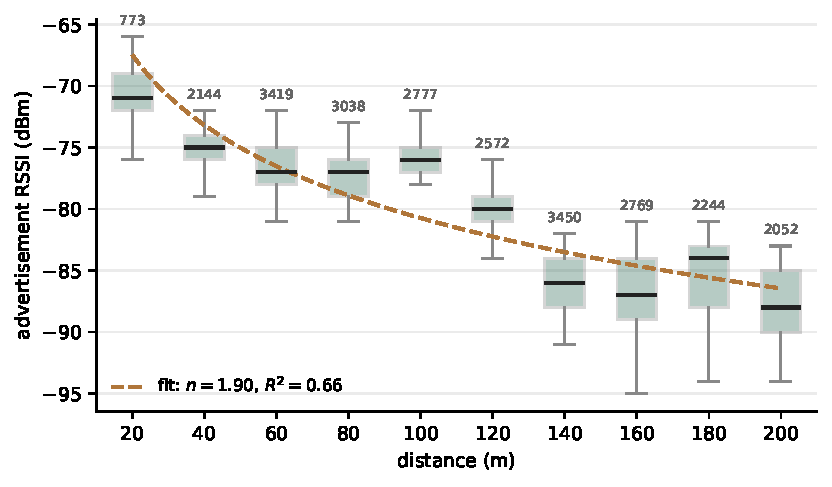
\includegraphics[width=\linewidth]{figures/line200_path_loss.pdf}
    \captionof{figure}{Path loss vs. distance}
    \column{0.42\textwidth}
    \raggeditems
    \begin{itemize}
        \item Compare to Rappaport standard path-loss model for 5G waves~\cite{Rappaport2013}
        \item Two Nexus 5X from 20 to 200\,m in 20\,m steps; ten cold-start runs per point, 100 messages each way
    \end{itemize}
    \end{columns}
    \takeaway{$\mathrm{RSSI}(d) = -43.5 - 18.8\log_{10} d$, exponent $n \approx 1.9$, residual $\sigma = 3.6$\,dB}
\end{frame}
\begin{frame}{Experiment 1, the line: time to each stage}
    \centering
    \resizebox{0.95\textwidth}{!}{%
    \begin{tikzpicture}[x=1mm,y=1mm, font=\footnotesize,
                stage/.style={draw, thick, rounded corners=1pt, fill=white, align=center, minimum height=7mm, text width=19mm, inner sep=1pt},
                tr/.style={font=\scriptsize, text=black!60, align=center, text width=21mm},
                tm/.style={font=\small\bfseries, text=TUMBlue}]
                \foreach \i/\stg/\med/\how in {
                    0/{1. Advertisement\\seen}/{1.03 s}/{scanner hears the\\peripheral},
                    1/{2. Connection\\established}/{1.55 s}/{central connects,\\MTU negotiated},
                    2/{3. Peer\\identified}/{2.39 s}/{ANNOUNCE arrives},
                    3/{4. Secure session\\established}/{2.59 s}/{Noise XX handshake\\completes},
                    4/{5. Link\\usable}/{2.70 s}/{first payload\\delivered and ACK'd}} {
                    \node[stage] (s\i) at (\i*24+10,0) {\stg};
                    \node[tm, below=0.8mm of s\i] {\med};
                    \node[tr, above=0.8mm of s\i] {\how};
                }
                \foreach \i [evaluate=\i as \j using int(\i+1)] in {0,...,3} {\draw[->, thick] (s\i) -- (s\j);}
                % \node[font=\scriptsize, text=black!60, anchor=north, align=center] at (58,-8.5) {Median time from a cold start on a Nexus 5X pair. Stage 6, \emph{link settled}: the reverse leg repeats 1--4 in parallel.};
            \end{tikzpicture}}
    \captionof{figure}{The five link stages, with median time from a cold start}
    \begin{itemize}
        \item Discovery is bound by the radio; every later stage is paid for by the application
    \end{itemize}
    \takeaway{Identifying the peer is the costliest app step at 0.84\,s, the Noise handshake adds only 0.2\,s.}
\end{frame}

\begin{frame}{Experiment 1, the line: bytes to each stage}
    \begin{columns}[T]
    \column{0.50\textwidth}
    \centering
    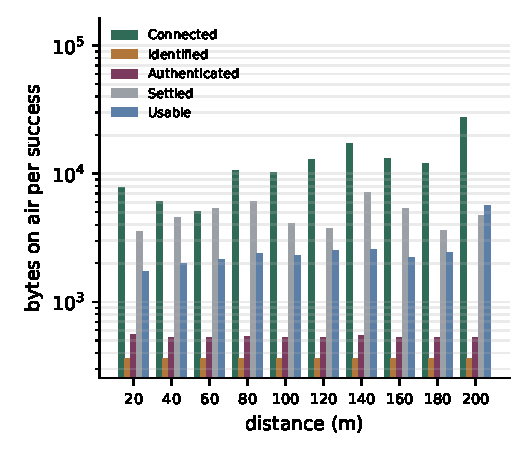
\includegraphics[width=0.96\linewidth]{figures/line200_stage_bytes_rungs.pdf}
    \captionof{figure}{Bytes to each stage, by distance}
    \column{0.50\textwidth}
    \centering
    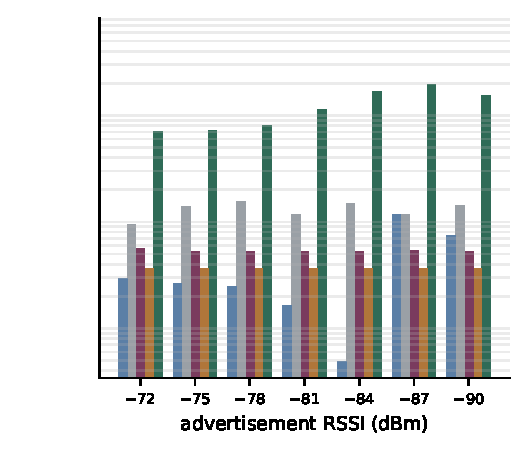
\includegraphics[width=0.96\linewidth]{figures/line200_stage_bytes_rungs_rssi.pdf}
    \captionof{figure}{The same runs, by RSSI}
    \end{columns}
    \begin{itemize}
        \item Advertising dominates the other stages: reaching a GATT link costs up to 27\,kB at a 135\,ms advertisement interval, followed by session (524 B) and identity (364 B)
        % \item Identity then costs 364\,B (two ANNOUNCEs) and a session 524\,B (four packets), both flat across RSSI
    \end{itemize}
    \takeaway{Finding the peer is what costs bytes; the secure session itself is nearly free.}
\end{frame}

\begin{frame}{Experiment 2, the diluting clique: contention collapses delivery}
    \begin{columns}[T]
    \column{0.58\textwidth}
    \centering
    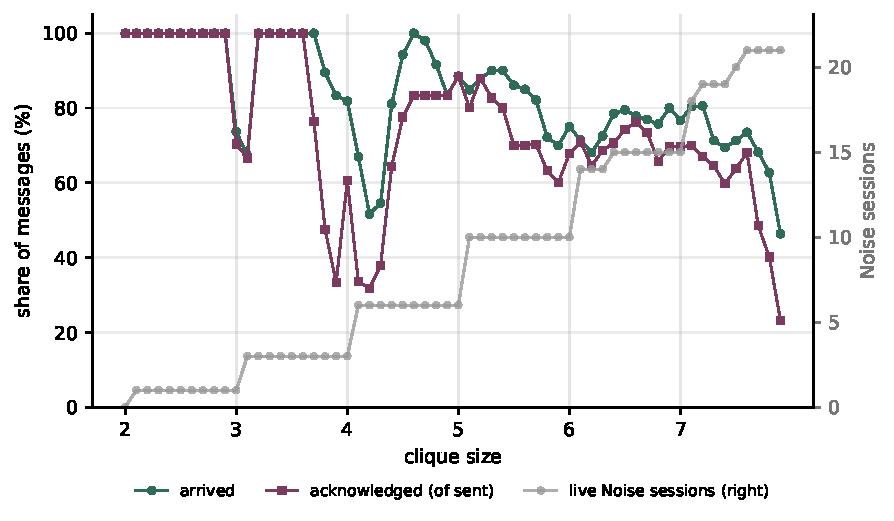
\includegraphics[width=\linewidth]{figures/clique_delivery_per_trial.pdf}
    \captionof{figure}{Delivery and ACKs per trial as the clique grows}
    \column{0.40\textwidth}
    \raggeditems
    \begin{itemize}
        \item The clique grows from 2 to 7 phones within 30\,m; offered load rises from 6.7 to 140 msg/s
        \item Delivery falls from 100\,\% to 50\,\%, ACKs to 20\,\%, median latency from 110\,ms to 9\,s
        \item Each join degrades delivery, as all nodes spend airtime on link establishment
    \end{itemize}
    \end{columns}
    \takeaway{Radio contention and hardware, not the range, are the constraints: every pair sat at a lossless RSSI.}
\end{frame}

\begin{frame}{Experiment 3, link flapping: frequent link loss, heavy-tailed outages}
    \begin{columns}[T]
    \column{0.32\textwidth}
    \centering
    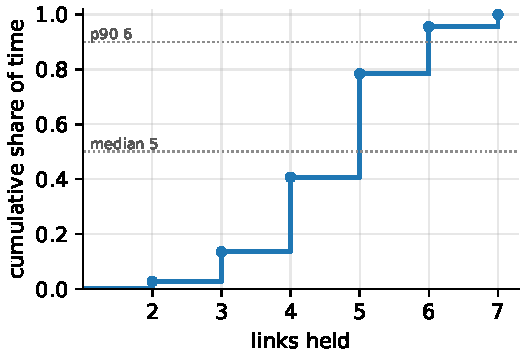
\includegraphics[height=2.6cm]{figures/churn_links_held_cdf.pdf}
    \captionof{figure}{Links held, CDF}
    \column{0.32\textwidth}
    \centering
    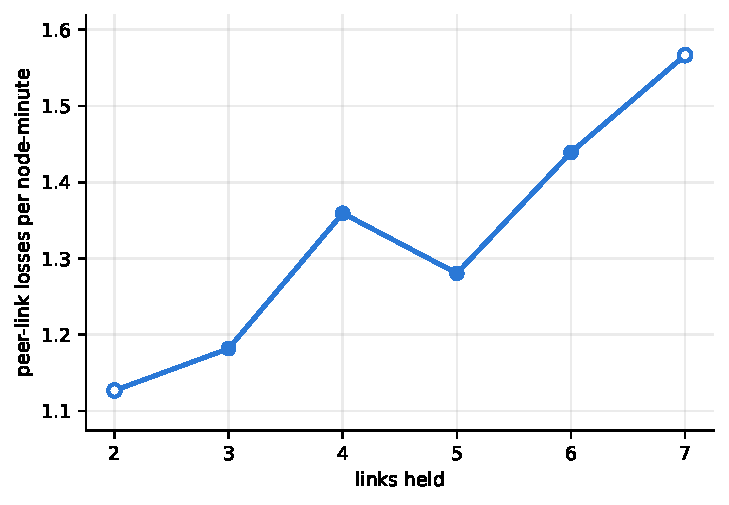
\includegraphics[height=2.6cm]{figures/churn_rate_by_degree.pdf}
    \captionof{figure}{Link loss rate vs. links held}
    \column{0.32\textwidth}
    \centering
    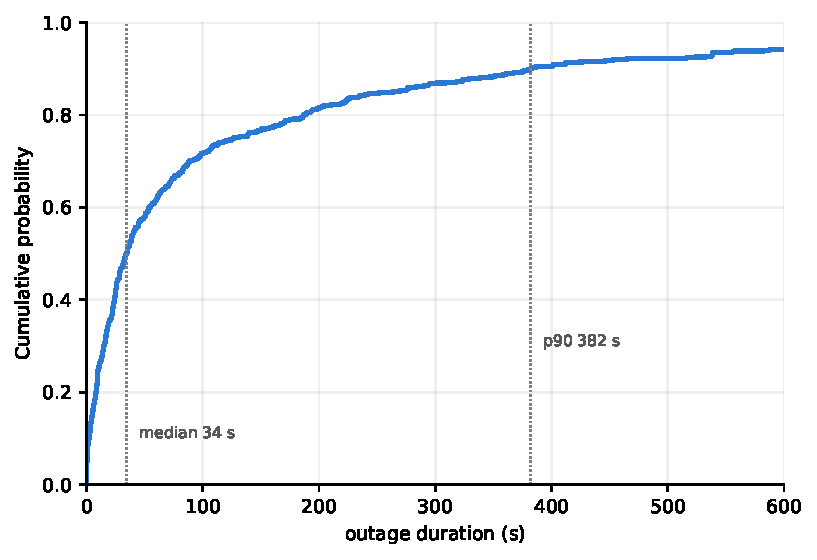
\includegraphics[height=2.6cm]{figures/churn_outage.pdf}
    \captionof{figure}{Outage duration, CDF}
    \end{columns}
    \begin{itemize}
        \item Eight phones at short range with sessions established beforehand: only physical link loss is measured
        % \item Links held by a Nexus 5X: median 5, p90 6, range 2 to 7, mean 4.7 (it sits at the 7-link cap only 4.5\,\% of the time)
        % \item Outages: median 34\,s, p90 382\,s, maximum 5\,356\,s
    \end{itemize}
    \takeaway{These distributions calibrate the simulation.}
\end{frame}

\begin{frame}{Simulations: congestion at scale}
    \begin{columns}[T]
    \column{0.44\textwidth}
    \begin{center}
        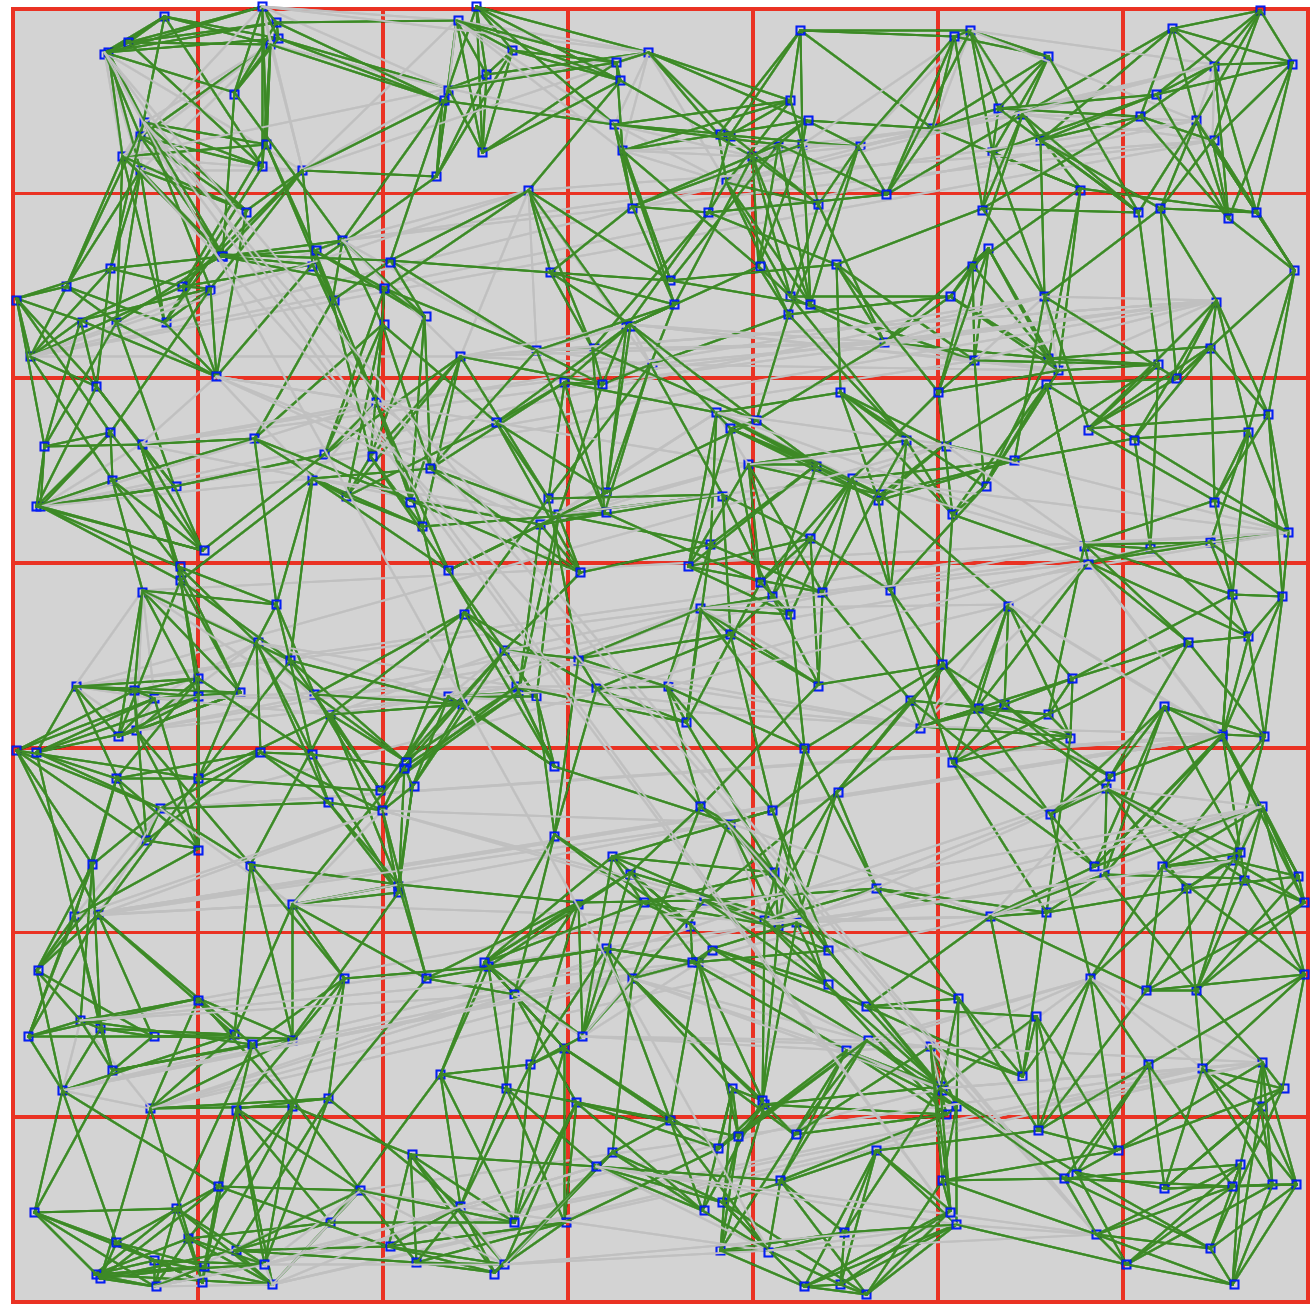
\includegraphics[width=\linewidth]{pics/sim-hall-topology.png}
    \end{center}
    \vspace{-1ex}
    {\footnotesize Red: the 49 cells of 50\,m, 8 nodes each. Green: the lanes messages flood on; grey: links held but passive}
    \column{0.54\textwidth}
    \raggeditems
    \textbf{Scenario in the ONE~\cite{the-one}}
    \begin{itemize}
        \item 350\,$\times$\,350\,m hall, 49 cells, 8 nodes per cell: 392 nodes
        \item 50\,m radio range (lossless), at most 7 links per node
        \item One new message per second for 30\,000\,s; 25 seeded placements per arm
    \end{itemize}
    \vspace{0.5ex}
    \textbf{Five control-plane establishment strategies}\\[0.5ex]
    \scriptsize
    \setlength{\tabcolsep}{4pt}
    \begin{tabular}{@{}lY{4.8cm}@{}}
        \toprule
        \texttt{flood} & epidemic flooding, as in GNL and BitChat \\
        \texttt{f3} & flood only the top 3 links by ego-network centrality~\cite{Daly2007} and buffer occupancy \\
        \texttt{oracle} & omniscient shortest path: the BLE ceiling \\
        \texttt{amigo} & leader-elected territories, after Amigo's dynamic clique routing~\cite{Inyangson2025} \\
        \texttt{amigo-udx} & \texttt{amigo} plus UDX between leaders, at the 2.4\,MB/s measured on a Nexus 5X \\
        \bottomrule
    \end{tabular}
    \end{columns}
\end{frame}

\begin{frame}{Simulations: the model the arms run on}
    % \begin{moepdef}{blue}{filled}{}
    %     \textbf{Link flapping, calibrated on experiment 3.} Every $\Delta t = 30$\,s a node $u$ holding $k_u$ links drops $D_u \sim \mathrm{Pois}\big(\lambda(k_u)\,\Delta t\big)$ of them, chosen uniformly. The measured rate depends on the links held, and the two directions differ: \emph{per node} it rises, $\lambda(k) = 1.13,\ 1.18,\ 1.36,\ 1.28,\ 1.44,\ 1.57$ per node-minute for $k = 2\ldots 7$, while \emph{per link} $\lambda(k)/k$ falls from $0.57$ to $0.22$. Endpoints draw independently, so link $i$--$j$ flaps at
    %     \[
    %         \lambda_{ij} \;=\; \frac{\lambda(k_i)}{k_i} + \frac{\lambda(k_j)}{k_j}
    %         \qquad\quad k_i = k_j = 7:\;\; \lambda_{ij} \approx 0.45\,\text{min}^{-1}, \text{ mean time between flaps 2.2 min}
    %     \]
    %     and stays down at both ends for a resampled measured outage: heavy-tailed, median $\approx$ 35\,s.
    % \end{moepdef}
    \begin{moepdef}{blue}{filled}{}
        \textbf{Link flapping, calibrated on experiment 3.} Every $\Delta t = 30$\,s a node $u$ holding $k_u$ links drops $D_u \sim \mathrm{Pois}\big(\lambda(k_u)\,\Delta t\big)$ of them, chosen uniformly. Endpoints draw independently, so link $i$--$j$ flaps at
        \[
            \lambda_{ij} \;=\; \frac{\lambda(k_i)}{k_i} + \frac{\lambda(k_j)}{k_j}
            \qquad\quad k_i = k_j = 7:\;\; \lambda_{ij} \approx 0.45\,\text{min}^{-1}, \text{ mean time between flaps 2.2 min}
        \]
        and stays down at both ends for a resampled measured outage: heavy-tailed, median $\approx$ 35\,s.
    \end{moepdef}
\end{frame}

\begin{frame}{Simulations: only the wide-area underlay overcomes the hop limit}
    \begin{center}
        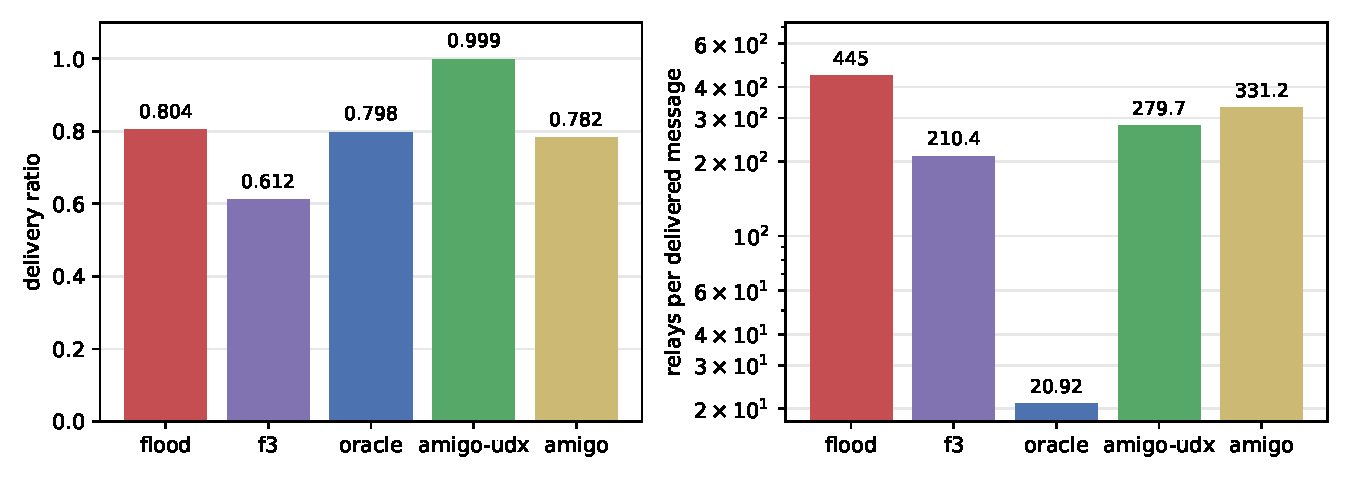
\includegraphics[width=0.86\textwidth]{figures/sim_reach_ceiling.pdf}
        \captionof{figure}{Delivery ratio and relays per delivered message, five arms}
    \end{center}
    \begin{itemize}
        \item \texttt{flood} and \texttt{oracle} both deliver about 80\,\%: the hop limit of 7 bounds reachability. Flooding costs 445 relays per delivered message, the oracle 21
        \item \texttt{f3} halves the relays but falls to 61\,\%; \texttt{amigo} on BLE alone reaches 78\,\% at near-flood cost
        \item \texttt{amigo-udx} delivers 99.9\,\% with a third fewer relays than flooding and the lowest buffer occupancy
    \end{itemize}
    \takeaway{A BLE-only mesh does not scale to this network, not even with optimal routing. Rendezvous points should be used as backbone to deliver messages across the network.}
\end{frame}
